\section{TẬP HỢP}

\subsection{TÓM TẮT LÝ THUYẾT}

\subsubsection{Nhắc lại về tập hợp}
\begin{enumerate}[\iconMT]
	\item \indam{Tập hợp}
	\begin{enumerate}[\faPencilSquareO]
		\item Khi muốn mô tả các đối tượng (phần tử) có chung một tính chất gì đó thì ta xây dựng khái niệm tập hợp.
		\begin{boxkn}
		\begin{itemize}
			\item  Người ta thường dùng chữ cái in hoa $A$, $B$, $\cdots$ để kí hiệu tập hợp.
			\item  Để chỉ $a$ thuộc tập hợp $A$, ta viết $a \in A$; để chỉ $a$ không thuộc tập hợp $A$, ta viết $a \notin A$.
			\item Số phần tử của tập $A$ được kí hiệu là $n(A)$.
		\end{itemize}
		\end{boxkn}
		\item Cách xác định tập hợp: 
		\begin{boxkn}
		\begin{itemize}
			\item  Liệt kê các phần tử: viết các phần tử của tập hợp trong hai dấu ngoặc nhọn $\left\{...\right\}$.
			\item  Chỉ ra tính chất đăc trưng cho các phần tử của tập hợp.
		\end{itemize}
		\end{boxkn}
		\item Tập rỗng: là tập hợp không chứa phần tử nào, kí hiệu $\varnothing $.
	\end{enumerate}	
	\item \indam{Các tập hợp số}
	\begin{listEX}[2]
		\item [\ding{172}] Tập số tự nhiên $\mathbb{N}$.
		\item [\ding{173}] Tập số nguyên $\mathbb{Z}$.
		\item [\ding{174}] Tập số hữu tỉ $\mathbb{Q}$.
		\item [\ding{175}] Tập số vô tỉ $\mathbb{I}$.
		\item [\ding{176}] Tập số thực $\mathbb{R}$.
		\item [\ding{177}] Tập $\mathbb{N}^{}$: tập hợp các số tự nhiên khác $0$
	\end{listEX}
\end{enumerate}
\subsubsection {Tập con và hai tập hợp bằng nhau}
Cho hai tập hợp $A$ và $B$
	\begin{enumerate}[\iconMT]
		\item \indam{Tập hợp con:}  Nếu mọi phần tử của $A$ đều nằm trong $B$ thì ta nói tập $A$ là con của tập $B$, nghĩa là $$A\subset B\Leftrightarrow (\forall x\colon x \in A\Rightarrow x\in B)$$
		\begin{tcolorbox}[colframe=cyan,colback=white,boxrule=0.2mm]
			\immini{\begin{itemize}
					\item  Các tính chất:
					\begin{listEX}[1]
						\item [\ding{172}] $A\subset A,\forall A$.
						\item [\ding{173}] $\varnothing \subset A,\forall A$.
						\item [\ding{174}] $A\subset B$, và $B\subset C$ suy ra $A\subset C$.
					\end{listEX}
				\item  Nếu $A$ không phải tập con của $B$ thì ta kí hiệu $A\not\subset B$.
				\item Nếu $A \subset B$ hoặc $B \subset A$ thì ta nói $A$ và $B$ có quan hệ bao hàm.
			\end{itemize}}{
				\begin{tikzpicture}[smooth,font=\footnotesize,scale=1]
					\def\miena{(0,0) to[bend left=90] (2,2) to[bend left=90] (0,0)}
					\def\mienb{(0.5,0.5) to[bend left=90] (1.5,1.75) to[bend left=90] (0.5,0.5)}
					\draw[pattern=dots] \miena;
					\draw[fill=white] \mienb
					(1,-0.7) node{Biểu đồ Ven minh họa $A \subset B$}
					(1,1.2) node{$A$}
					(0.5,0.1) node{$B$};
			\end{tikzpicture}}
		\end{tcolorbox}
		\indamm{Mối quan hệ giữa các tập hợp số:}
		\begin{listEX}[2]
			\item [\ding{172}] $\mathbb{N} \subset \mathbb{Z} \subset \mathbb{Q} \subset \mathbb{R}$.
			\item [\ding{173}] $\mathbb{Q} \cup \mathbb{I}=\mathbb{R}$.
		\end{listEX}
		\item \indam{Tập hợp bằng nhau:} $A=B\Leftrightarrow A\subset B$ và $B\subset A\Leftrightarrow (\forall x \colon x\in A\Leftrightarrow x\in B)$.
		\end{enumerate}
\subsubsection{Một số tập con của tập hợp số thực}

	\begin{listEX}[2]
		\item [\ding{172}] Khoảng $\left(a;b\right)=\left\{\left. x\in \mathbb{R}\right|a<x<b\right\}$.\\
		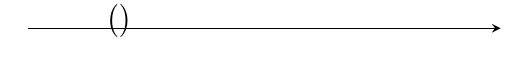
\begin{tikzpicture}[>=stealth]
			\draw[->](-1,0)->(5,0);
			\IntervalLR{-1}{1/2}
			\def\skipInterval{0.5cm}%Khoảng cách đặt nhãn
			\IntervalGRF{}{}{\big(}{a}%Gạch xọc phải qua trái
			\IntervalLR{4}{4.8}
			\def\skipInterval{0.5cm}%Khoảng cách đặt nhãn
			\IntervalGRF{\big)}{b}{}{}%Gạch xọc phải qua trái
		\end{tikzpicture}	
		\item [\ding{173}] Đoạn $\left[a;b\right]=\left\{\left. x\in \mathbb{R}\right|a\le x\le b\right\}$.\\
		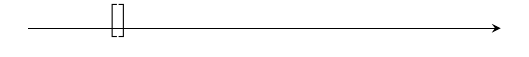
\begin{tikzpicture}[>=stealth]
			\draw[->](-1,0)->(5,0);
			\IntervalLR{-1}{1/2}
			\def\skipInterval{0.5cm}%Khoảng cách đặt nhãn
			\IntervalGRF{}{}{\big[}{a}%Gạch xọc phải qua trái
			\IntervalLR{4}{4.8}
			\def\skipInterval{0.5cm}%Khoảng cách đặt nhãn
			\IntervalGRF{\big]}{b}{}{}%Gạch xọc phải qua trái
		\end{tikzpicture}
		\item [\ding{174}] Khoảng $\left(a;+\infty \right)=\left\{\left. x\in \mathbb{R}\right|x>a\right\}$.\\
		\begin{tikzpicture}[>=stealth]
			\draw[->](-1,0)--(5,0)node[below]{$+\infty$};
			\IntervalLR{-1}{1/2}
			\def\skipInterval{0.5cm}%Khoảng cách đặt nhãn
			\IntervalGRF{}{}{\big(}{a}%Gạch xọc phải qua trái
			\IntervalLR{4}{4.8}
			\def\skipInterval{0.5cm}%Khoảng cách đặt nhãn
			%\IntervalGRF{\big]}{b}{}{}%Gạch xọc phải qua trái
		\end{tikzpicture}
		\item [\ding{175}] Nửa khoảng $\left[a;+\infty \right)=\left\{\left. x\in \mathbb{R}\right|x\ge a\right\}$.\\
		\begin{tikzpicture}[>=stealth]
			\draw[->](-1,0)->(5,0)node[below]{$+\infty$};
			\IntervalLR{-1}{1/2}
			\def\skipInterval{0.5cm}%Khoảng cách đặt nhãn
			\IntervalGRF{}{}{\big[}{a}%Gạch xọc phải qua trái
			\IntervalLR{4}{4.8}
			\def\skipInterval{0.5cm}%Khoảng cách đặt nhãn
			%\IntervalGRF{\big]}{b}{}{}%Gạch xọc phải qua trái
		\end{tikzpicture}
		\item [\ding{176}] Khoảng $\left(-\infty;b\right)=\left\{\left. x\in \mathbb{R}\right|x<b\right\}$.\\
		\begin{tikzpicture}[>=stealth]
			\draw[->](-1,0)node[below]{$-\infty$}--(5,0);
			\IntervalLR{-1}{1/2}
			\def\skipInterval{0.5cm}%Khoảng cách đặt nhãn
			%\IntervalGRF{}{}{\big[}{a}%Gạch xọc phải qua trái
			\IntervalLR{3}{4.8}
			\def\skipInterval{0.5cm}%Khoảng cách đặt nhãn
			\IntervalGRF{\big)}{b}{}{}%Gạch xọc phải qua trái
		\end{tikzpicture}
		\item [\ding{177}] Nửa khoảng $\left(-\infty;b\right]=\left\{\left. x\in \mathbb{R}\right|x\le b\right\}$.\\
		\begin{tikzpicture}[>=stealth]
			\draw[->](-1,0)node[below]{$-\infty$}->(5,0);
			\IntervalLR{-1}{1/2}
			\def\skipInterval{0.5cm}%Khoảng cách đặt nhãn
			%\IntervalGRF{}{}{\big[}{a}%Gạch xọc phải qua trái
			\IntervalLR{3}{4.8}
			\def\skipInterval{0.5cm}%Khoảng cách đặt nhãn
			\IntervalGRF{\big]}{b}{}{}%Gạch xọc phải qua trái
		\end{tikzpicture}
		\item [\ding{178}] Nửa khoảng $\left[a;b\right)=\left\{\left. x\in \mathbb{R}\right|a\le x<b\right\}$.\\
		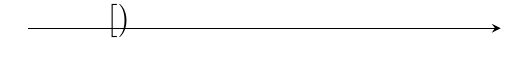
\begin{tikzpicture}[>=stealth]
			\draw[->](-1,0)->(5,0);
			\IntervalLR{-1}{1/2}
			\def\skipInterval{0.5cm}%Khoảng cách đặt nhãn
			\IntervalGRF{}{}{\big[}{a}%Gạch xọc phải qua trái
			\IntervalLR{4}{4.8}
			\def\skipInterval{0.5cm}%Khoảng cách đặt nhãn
			\IntervalGRF{\big)}{b}{}{}%Gạch xọc phải qua trái
		\end{tikzpicture}
		\item [\ding{179}] Nửa khoảng $\left(a;b\right]=\left\{\left. x\in \mathbb{R}\right|a<x\le b\right\}$.\\
		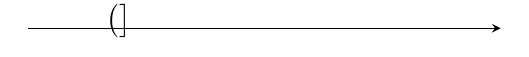
\begin{tikzpicture}[>=stealth]
			\draw[->](-1,0)->(5,0);
			\IntervalLR{-1}{1/2}
			\def\skipInterval{0.5cm}%Khoảng cách đặt nhãn
			\IntervalGRF{}{}{\big(}{a}%Gạch xọc phải qua trái
			\IntervalLR{4}{4.8}
			\def\skipInterval{0.5cm}%Khoảng cách đặt nhãn
			\IntervalGRF{\big]}{b}{}{}%Gạch xọc phải qua trái
		\end{tikzpicture}
	\end{listEX}
\subsection{RÈN LUYỆN KĨ NĂNG GIẢI TOÁN}
\begin{dang}{Xác định tập hợp}
\end{dang}

\begin{vd}%[0D1Y2-1]
	Cho $D=\{n \in \mathbb{N} \mid n$ là số nguyên tố, $5<n<20\}$.
	\begin{enumEX}{1}
		\item Viết tập hợp $D$ bằng cách liệt kê các phần tử. Tập hợp $D$ có bao nhiêu phần tử?
		\item Dùng kí hiệu $\in, \notin$ để viết câu trả lời cho câu hỏi sau: Trong các số $5$; $12$; $17$; $18$, số nào thuộc tập $D$, số nào không thuộc tập $D$?
	\end{enumEX}
	\loigiai{
		\begin{enumEX}{1}
			\item $D=\{7 ; 11 ; 13 ; 17 ; 19\}$. Tập hợp $D$ có $5$ phần tử.
			\item $5 \notin D$; $12 \notin D$; $17 \in D$; $18 \notin D$.
		\end{enumEX}	
	}
\end{vd}\dongcham{2}

\begin{ex}
	Viết mỗi tập hợp sau bằng cách liệt kê các phần tử.
	\begin{enumEX}[a)]{2}
		\item $A = \{x \in \mathbb{Z} \mid 2x^2 - 75x - 77 = 0\}$.
		\item $B = \{x \in \mathbb{Z} \mid 2x^3 - 3x^2 - 5x = 0\}$.
		\item $C = \{x \in \mathbb{R} \mid (2x - x^2)(3x - 2) = 0\}$.
		\item $D = \{x \in \mathbb{R} \mid (x^2 - x - 2)(x^2 - 9) = 0\}$.
	\end{enumEX}
	\loigiai{
		\begin{enumerate}
			\item[a)] Xét phương trình:
			$$ 2x^2 - 75x - 77 = 0 \Leftrightarrow \left[ \begin{aligned} &x = -1 \\ &x = \frac{77}{2} \end{aligned} \right. $$
			Vì điều kiện $x \in \mathbb{Z}$ (chỉ lấy các số nguyên) nên ta loại $x = \frac{77}{2}$, chỉ nhận nghiệm $x = -1$.\\
			Vậy $A = \{-1\}$.
			
			\item[b)] Xét phương trình:
			$$ 2x^3 - 3x^2 - 5x = 0 \Leftrightarrow x(2x^2 - 3x - 5) = 0 \Leftrightarrow \left[ \begin{aligned} &x = 0 \\ &2x^2 - 3x - 5 = 0 \end{aligned} \right. \Leftrightarrow \left[ \begin{aligned} &x = 0 \\ &x = -1 \\ &x = \frac{5}{2} \end{aligned} \right. $$
			Vì điều kiện $x \in \mathbb{Z}$ nên ta chỉ nhận các nghiệm nguyên là $x = 0$ và $x = -1$.\\
			Vậy $B = \{-1; 0\}$.
			
			\item[c)] Xét phương trình:
			$$ (2x - x^2)(3x - 2) = 0 \Leftrightarrow \left[ \begin{aligned} &2x - x^2 = 0 \\ &3x - 2 = 0 \end{aligned} \right. \Leftrightarrow \left[ \begin{aligned} &x = 0 \\ &x = 2 \\ &x = \frac{2}{3} \end{aligned} \right. $$
			Vì điều kiện $x \in \mathbb{R}$ (tập hợp số thực) nên ta nhận tất cả các nghiệm trên.\\
			Vậy $C = \left\{0; \frac{2}{3}; 2\right\}$.
			
			\item[d)] Xét phương trình:
			$$ (x^2 - x - 2)(x^2 - 9) = 0 \Leftrightarrow \left[ \begin{aligned} &x^2 - x - 2 = 0 \\ &x^2 - 9 = 0 \end{aligned} \right. \Leftrightarrow \left[ \begin{aligned} &x = -1 \\ &x = 2 \\ &x = 3 \\ &x = -3 \end{aligned} \right. $$
			Vì điều kiện $x \in \mathbb{R}$ nên ta nhận tất cả các nghiệm thu được.\\
			Vậy $D = \{-3; -1; 2; 3\}$.
		\end{enumerate}
	}
\end{ex}
\dongcham{4}
\begin{vd}
	Viết các tập hợp sau đây dưới dạng liệt kê các phần tử:
	\begin{enumEX}[a)]{2}
		\item $A = \{x \mid x^2 - 2x - 15 = 0\}$;
		\item $B = \{x \in \mathbb{Z} \mid -3 < x \le 2\}$;
		\item $C = \left\{\dfrac{n}{n^2 - 1} \mid n \in \mathbb{N}, 1 < n \le 4\right\}$;
		\item $D = \{(x; y) \mid x \le 2, y < 2, x, y \in \mathbb{N}\}$.
	\end{enumEX}
	\loigiai{
		\begin{enumerate}
			\item[a)] Ta xét phương trình: 
			$$ x^2 - 2x - 15 = 0 \Leftrightarrow \left[ \begin{aligned} &x = 5 \\ &x = -3 \end{aligned} \right. $$
			Vì tập $A$ không có điều kiện ràng buộc nào khác về tập hợp số (ngầm hiểu $x \in \mathbb{R}$), nên cả hai nghiệm đều thỏa mãn.\\
			Vậy $A = \{-3; 5\}$.
			
			\item[b)] Các số nguyên $x$ thỏa mãn điều kiện $-3 < x \le 2$ là: $-2; -1; 0; 1; 2$.\\
			Vậy $B = \{-2; -1; 0; 1; 2\}$.
			
			\item[c)] Các số tự nhiên $n$ thỏa mãn điều kiện $1 < n \le 4$ là: $2; 3; 4$. Thay lần lượt các giá trị này vào biểu thức $\dfrac{n}{n^2 - 1}$:
			\begin{itemize}
				\item Với $n = 2 \Rightarrow \dfrac{2}{2^2 - 1} = \dfrac{2}{3}$.
				\item Với $n = 3 \Rightarrow \dfrac{3}{3^2 - 1} = \dfrac{3}{8}$.
				\item Với $n = 4 \Rightarrow \dfrac{4}{4^2 - 1} = \dfrac{4}{15}$.
			\end{itemize}
			Vậy $C = \left\{\dfrac{2}{3}; \dfrac{3}{8}; \dfrac{4}{15}\right\}$.
			
			\item[d)] Tập hợp $D$ gồm các cặp số $(x; y)$ với $x, y \in \mathbb{N}$.\\
			Vì $x \le 2 \Rightarrow x \in \{0; 1; 2\}$.\\
			Vì $y < 2 \Rightarrow y \in \{0; 1\}$.\\
			Ghép các giá trị của $x$ và $y$ ta được các cặp số: $(0; 0), (0; 1), (1; 0), (1; 1), (2; 0), (2; 1)$.\\
			Vậy $D = \{(0; 0), (0; 1), (1; 0), (1; 1), (2; 0), (2; 1)\}$.
		\end{enumerate}
	}
\end{vd}
\dongcham{10}
\begin{vd}%[0D1K2-1]
	Viết mỗi tập hợp sau bằng cách nêu tính chất đặc trưng.
	\begin{enumEX}{2}
		\item $A=\{2;3;5;7\}$.
		\item $B=\{-3;-2;-1;0;1;2;3\}$.
		\item $C=\{-5;0;5;10\}$.
		\item $D=\{1;2;3;4;6;9;12;18;36\}$.
	\end{enumEX}
	\loigiai{
		\begin{enumerate}
			\item $A=\left\{x\in \mathbb{R}\big|\right. x$ nguyên tố và $\left.x<10\right\}$.
			\item $B=\left\{x\in \mathbb{Z}\big||x|\leqslant 3 \right\}$.
			\item $C=\left\{x\in \mathbb{Z}\big| x\vdots 5,-5\leqslant x\leqslant 10 \right\}$.
			\item $D=\left\{n\in \mathbb{N}\big|x \text{ là ước của } 36\right\}$.
		\end{enumerate}
	}
\end{vd}\dongcham{8}

\begin{vd}
	Trong các tập hợp sau, tập hợp nào rỗng?
	\begin{enumEX}{2}
		\item $A=\left\{\left. x\in \mathbb{R}\right|x^2-x+1=0\right\}$.
		\item $B=\left\{\left. x\in \mathbb{Q}\right|\right.x^2-4x+2\left. =0\right\}$.
		\item $C=\left\{\left. x\in \mathbb{Z}\right|\right.6x^2-7x+1\left. =0\right\}$.
		\item $D=\left\{\left. x\in \mathbb{Z}\right|\right.\left| x\right|<\left. 1\right\}$.
	\end{enumEX}
	\loigiai{
		\begin{enumEX}{1}
			\item Phương trình $x^2-x+1=0$ có $\Delta <0$ nên vô nghiệm. Do đó $A=\varnothing $.
			\item Phương trình $x^2-4x+2=0$ có hai nghiệm $x=2\pm \sqrt{2}\notin \mathbb{Q}$. Do đó $B=\varnothing $.
			\item Phương trình $6x^2-7x+1=0$ có nghiệm $x=1\in \mathbb{Z}$. Do đó $C\ne \varnothing $.
			\item Chọn $x=0\in \mathbb{Z},\left| 0\right|<1$. Do đó $D\ne \varnothing $.
		\end{enumEX}
	}
\end{vd}\dongcham{8}

\begin{dang}{Xác định tập hợp con. Hai tập hợp bằng nhau}
	Cho tập hợp $A$ gồm $n$ phần tử.
	\begin{listEX}[1]
		\item [\ding{172}] Khi liệt kê tất cả các tập con của $A$, ta liệt kê đầy đủ theo thứ tự:\\		
		\centerline{ $\varnothing$; tập $1$ phần tử; tập $2$ phần tử; tập $3$ phần tử;...; $A$.}
		\item [\ding{173}] Số tập con của $A$ là $2^n$.
		\item [\ding{174}] Số tập con gồm $k$ phần tử của $A$ là $\mathrm{C}_n^k$ (dùng để kiểm tra kết quả bằng máy tính).
	\end{listEX}
\end{dang}
\begin{vd}
	Cho tập hợp $A = \{2; 3; 4\}$ và $B = \{2; 3; 4; 5; 6\}$.
	\begin{enumerate}
		\item[a)] Xác định tất cả tập con có hai phần tử của $A$.
		\item[b)] Xác định tất cả tập con có ít hơn hai phần tử của $A$.
		\item[c)] Tập $A$ có tất cả bao nhiêu tập con?
		\item[d)] Xác định tất cả các tập $X$ thỏa $A \subset X \subset B$.
	\end{enumerate}
	\loigiai{
		\begin{enumerate}
			\item[a)] Các tập hợp con có hai phần tử của $A$ là: $\{2; 3\}$, $\{2; 4\}$, $\{3; 4\}$.
			\item[b)] Các tập hợp con có ít hơn hai phần tử của $A$ (bao gồm tập rỗng và tập có một phần tử) là: $\varnothing$, $\{2\}$, $\{3\}$, $\{4\}$.
			\item[c)] Tập hợp $A$ có $3$ phần tử. Do đó, số lượng tập con của tập hợp $A$ là: $2^3 = 8$ (tập con).
			\item[d)] Vì $A \subset X \subset B$ nên tập hợp $X$ phải chứa toàn bộ các phần tử của tập hợp $A=\{2; 3; 4\}$, đồng thời các phần tử cấy thêm vào $X$ (nếu có) phải được lấy từ tập hợp $\{5; 6\}$.\\
			Các tập hợp $X$ thỏa mãn yêu cầu bài toán là:
			\begin{itemize}
				\item $X_1 = \{2; 3; 4\}$
				\item $X_2 = \{2; 3; 4; 5\}$
				\item $X_3 = \{2; 3; 4; 6\}$
				\item $X_4 = \{2; 3; 4; 5; 6\}$
			\end{itemize}
		\end{enumerate}
	}
\end{vd}\dongcham{8}


\begin{vd}%[0D1B4-1]
	Cho hai tập hợp $A=\{a;b;c;d;e\}$ và $B=\{a;c;e;f\}$. Tìm tất cả các tập hợp $X$ sao cho $X\subset A$ và $X\subset B$.
	\loigiai{
		Ta có $\left\{\begin{aligned}
			&X\subset A\\
			&X\subset B
		\end{aligned}\right. $, suy ra phần tử của tập X thuộc tập $\{a;c;e\}$.\\
		Vậy các tập $X$ cần tìm là
		$$\varnothing, \{a\}, \{c\}, \{e\}, \{a;c\}, \{a;e\}, \{c;e\}, \{a;c;e\}$$
		
	}
\end{vd}\dongcham{6}

\begin{vd} 
	Cho hai tập hợp $A=\{1 ; a ; 5\}, B=\{a+2 ; 3 ; b\}$ với $a, b$ là các số thực. Biết rằng $A=B$, hãy xác định $a$ và $b$.
	\loigiai{Vì $3 \in B$ và $A=B$ nên ta có $3 \in A=\{1 ; a ; 5\}$, do đó, $a=3$. Khi đó, $B=\{5 ; 3 ; b\}$.\\
		Vì $1 \in A$ và $A=B$ nên ta có $1 \in B=\{5 ; 3 ; b\}$. Suy ra, ta có $b=1$.\\
		Khi đó, $A=B=\{1 ; 3 ; 5\}$. Vậy các giá trị cần tìm là $a=3, b=1$.
	}
\end{vd}\dongcham{6}

\begin{vd}
	Cho hai tập hợp $A = \left\{x \in \mathbb{Z} \mathrel{\Big|} \dfrac{2x+3}{x-1} \in \mathbb{Z}\right\}$ và $B = \{x \in \mathbb{Z} \mid x^2 - (m+2)x + 2m = 0\}$. Tìm tất cả các số nguyên $m$ sao cho $B \subset A$.
	\loigiai{
		\textbf{Bước 1:} Xác định các phần tử của tập $A$.\\
		Ta có $\dfrac{2x+3}{x-1} = \dfrac{2(x-1) + 5}{x-1} = 2 + \dfrac{5}{x-1}$.\\
		Để $\dfrac{2x+3}{x-1} \in \mathbb{Z}$ (với $x \in \mathbb{Z}$), thì $x-1$ phải là ước của $5$.\\
		Suy ra $x-1 \in \{-5; -1; 1; 5\} \Rightarrow x \in \{-4; 0; 2; 6\}$.\\
		Vậy $A = \{-4; 0; 2; 6\}$.
		
		\textbf{Bước 2:} Phân tích tập $B$.\\
		Xét phương trình $x^2 - (m+2)x + 2m = 0$.\\
		Ta có $\Delta = (m+2)^2 - 8m = m^2 - 4m + 4 = (m-2)^2 \ge 0$.\\
		Phương trình luôn có hai nghiệm: $x_1 = \dfrac{m+2 + m-2}{2} = m$ và $x_2 = \dfrac{m+2 - m+2}{2} = 2$.\\
		Suy ra $B = \{2; m\}$.
		
		\textbf{Bước 3:} Tìm điều kiện để $B \subset A$.\\
		Để $B \subset A$ thì mọi phần tử của $B$ đều phải thuộc $A$.
		Ta đã có $2 \in A$. Vậy điều kiện cần và đủ là $m \in A$.\\
		Suy ra $m \in \{-4; 0; 2; 6\}$.\\
		Kết hợp với điều kiện $m \in \mathbb{Z}$, ta nhận tất cả các giá trị này.
	}
\end{vd}
\dongcham{8}
\begin{dang}{Các tập con của tập số thực}
\end{dang}

\begin{vd}%[0D1B3]
	 Hãy dùng kí hiệu đoạn, khoảng, nửa khoảng để viết lại các tập hợp sau đây:
	 \begin{tasks}(2)
	 	\task $A=\left\lbrace  x\in \mathbb{R}\mid -1<x<5\right\rbrace$.
	 	\task $B=\left\lbrace  x\in \mathbb{R}\mid -1\le x < 5\right\rbrace$.
	 	\task $C=\left\lbrace  x\in \mathbb{R}\mid x \ge 4\right\rbrace$.
	 	\task $D=\left\lbrace  x\in \mathbb{R}\mid x \le -5\right\rbrace$.
	 	\task $E=\left\lbrace  x\in \mathbb{R}\mid x<0\right\rbrace$.
	 	\task $F=\left\lbrace  x\in \mathbb{R}\mid x>3\right\rbrace$.
	 	\task $E=\left\lbrace  x\in \mathbb{R}\mid \big|x\big| \le 4\right\rbrace$.
	 	\task $F=\left\lbrace  x\in \mathbb{R}\mid \big|x-1\big| < 9\right\rbrace$.
	 \end{tasks}
 	\loigiai{
 	\begin{enumerate}
 		\item[a)] $A = (-1; 5)$.
 		\item[b)] $B = [-1; 5)$.
 		\item[c)] $C = [4; +\infty)$.
 		\item[d)] $D = (-\infty; -5]$.
 		\item[e)] $E = (-\infty; 0)$.
 		\item[f)] $F = (3; +\infty)$.
 		\item[g)] Ta có bất phương trình: $|x| \le 4 \Leftrightarrow -4 \le x \le 4$.\\
 		Suy ra tập hợp là đoạn $E = [-4; 4]$.
 		\item[h)] Ta có bất phương trình: $|x - 1| < 9 \Leftrightarrow -9 < x - 1 < 9 \Leftrightarrow -8 < x < 10$.\\
 		Suy ra tập hợp là khoảng $F = (-8; 10)$.
 	\end{enumerate}
 }
\end{vd}\dongcham{8}

\begin{vd}%[0D1G3]
	Cho hai tập hợp $A = \left[ m; m + 2\right]; B =\left[ -1; 2\right]$. Tìm tất cả các giá trị thực của tham số $m$ để $A \subset B$.
	\loigiai{Để $A \subset B$ thì $\heva{& m \geq -1\\& m + 2 \leq 2} \Leftrightarrow \heva{& m \geq -1 \\ & m \leq 0}$.}
\end{vd}\dongcham{10}

\boxmini{BÀI TẬP TỔNG HỢP TỰ LUYỆN}
\begin{baitap}%[0D1B2-1]
	Liệt kê các phần tử của các tập hợp sau:
	\begin{enumerate}
		\item $A=\left\lbrace n\in \mathbb{N} \mid n<5\right\rbrace$.
		\item $B$ là tập hợp các số tự nhiên lớn hơn $0$ và nhỏ hơn $5$.
		\item $C=\left\lbrace x\in \mathbb{R}\mid (x-1)(x+2)=0\right\rbrace$.
	\end{enumerate}
	\loigiai{
		\begin{enumerate}
			\item $A=\left\lbrace 0;1;2;3;4\right\rbrace$.
			\item $B=\left\lbrace 1;2;3;4\right\rbrace$.
			\item Ta có $(x-1)(x+2)=0 \Leftrightarrow \hoac{&x=1\\&x=-2.}$\\
			Mà $x\in \mathbb{R}$ nên
			$C=\left\lbrace -2;1\right\rbrace$.
		\end{enumerate}
	}
\end{baitap}\cham{8}
\begin{baitap}%[0D1B2-1]
	Viết các tập hợp sau bằng phương pháp liệt kê các phần tử:
	\begin{tasks}(2)
		\task $A=\left\lbrace  x\in \mathbb{Q}\mid (x^2-2x+1)(x^2-5)=0\right\rbrace$.
		\task $B=\left\lbrace x \in \mathbb{N}\mid 5<x^2<40\right\rbrace$.
		\task $C=\left\lbrace x\in \mathbb{Z}\mid x^2<9\right\rbrace$.
		\task $D=\left\lbrace x\in \mathbb{R}\mid \left|2x+1\right|=5\right\rbrace$.
	\end{tasks}
	\loigiai{
		\begin{enumerate}[a)]
			\item Ta có $x\in A\Leftrightarrow\hoac{&x^2-2x+1=0\\&x^2-5=0}\Leftrightarrow\hoac{&x=1\in\mathbb{Q}\\&x=\pm\sqrt{5}\not\in \mathbb{Q}.}$\\
			Vậy $A=\left\lbrace 1\right\rbrace$.
			\item $B=\left\lbrace 3;4;5;6\right\rbrace$.
			\item $C=\left\lbrace -2;-1;0;1;2\right\rbrace$.
			\item Ta có $\left|2x+1\right|=5\Leftrightarrow \hoac{&x=2\\&x=-3.}$\\
			Vậy $C=\left\lbrace 2;-3\right\rbrace$.
		\end{enumerate}
	}
\end{baitap}\cham{15}


\begin{baitap}
Cho các tập hợp $A=\{1 ; 2 ; 3 ; 4 ; 5\}$ và $B=\{1 ; 3 ; 5 ; 7 ; 9\}$. Hãy tìm tập hợp $M$ có nhiều phần tử nhất thoả mãn $M \subset A$ và $M \subset B$.
\loigiai{
	$M=\{1;3;5\}$.
}
\end{baitap}\cham{10}

\begin{baitap} %[0D1B2-2]%
	Hãy xét quan hệ bao hàm các tập hợp sau:
	\begin{itemize}
		\item [] $A$ là tập hợp các tam giác.
		\item [] $B$ là tập hợp các tam giác đều.
		\item [] $C$ là tập hợp các tam giác cân.
	\end{itemize}
	\loigiai{
		Dễ dàng nhận thấy  $B \subset C \subset A$}
\end{baitap}\cham{10}

\begin{baitap}%[0D1B2-2]
	Cho tập $X=\{1;2;3;4;5;6;7\}$.
	\begin{listEX}[1]
		\item Hãy tìm tất cả các tập con của $X$ có chứa các phần tử $1$, $3$, $5$, $7$.
		\item Có bao nhiêu tập con của $X$ chứa đúng $2$ phần tử ?
	\end{listEX}
	\loigiai{
		\begin{enumerate}
			\item[a)] Các tập con của $X$ chứa có các phần tử 1, 3, 5, 7 được thành lập bằng cách thêm vào tập $\left\{1;3  ;5;7\right\}$ các phần tử còn lại của tập $X$. Do đó tất cả các tập con của $X$ có chứa các phần tử 1, 3, 5, 7 là: $\left\{1;3  ;5;7\right\}$, $\left\{1;3  ;5;7;2\right\}$, $\left\{1;3  ;5;7;4\right\}$, $\left\{1;3  ;5;7;6\right\}$, $\left\{1;3  ;5;7;2;4\right\}$, $\left\{1;3  ;5;7;2;6\right\}$, $\left\{1;3  ;5;7;4;6\right\}$ và $X$.
			\item[b)]  Giả sử tập cần tìm là $\{a;b\}$ với $a, b\in X$ $a\ne b$.
			\begin{itemize}
				\item Vì $X$ có $7$ phần tử nên có 7 cách chọn phần tử $a$.
				\item Sau khi chọn $a$ thì $X$ còn 6 phần tử, do đó với mỗi cách chọn $a$, ta có 6 cách chọn phần tử $b$ bnhư vậy có $7.6=42$ cặp $(a;b)$ theo cách chọn này.
			\end{itemize}
			Nhưng với cách chọn trên thì với hai phần tử bất kì $a, b$ ta đã chọn lặp lại hai lần đó là hai cặp $(a;b)$ và $(b;a)$.\\
			Do đó, có $\dfrac{42}{2}=21$ tập con của $X$ chứa đúng hai phần tử.
		\end{enumerate}
	}
\end{baitap}\cham{10}

\begin{baitap}
	Cho hai tập hợp $A=\{1 ; 2 ; a\}$ và $B=\left\{1 ; a^{2}\right\}$. Tìm tất cả các giá trị của $a$ sao cho $B \subset A$.
	\loigiai{Ta có $B \subset A$ nếu $a^{2}=1$ hoặc $a^{2}=2$ hoặc $a^{2}=a$.\\
		Từ đó tìm được các giá trị của $a$ là: $-\sqrt{2} ;-1 ; 0 ; 1 ; \sqrt{2}$.}
\end{baitap}\cham{8}

\begin{baitap}%[0D1K2]
	Tìm tất cả các giá trị nguyên của tham số  $m$ để tập hợp $\left(1;m\right)$ chứa đúng 2 số nguyên dương.
	\loigiai{
		Các số nguyên dương lớn hơn 1 sẽ là 2; 3; 4,... Suy ra, để $\left(1;m\right)$  chỉ chứa 1 số nguyên dương thì giá trị nguyên cần tìm của $m$ là $m=4$.
	}
\end{baitap}\cham{8}


\begin{baitap}%[Trịnh Văn Xuân, latex-k10]%[0D1B4-1]
	Cho hai tập hợp $A=[0;3]$ và $B=[a;a+2]$. Tìm $a$ để $B\subset A$.
	\loigiai{
		Điều kiện: $a\in \mathbb{R}$.\\
		Để $B\subset A$ khi và chỉ khi $\left\{\begin{aligned}
			&a\geqslant 0\\
			&a+2\leqslant 3
		\end{aligned}\right. \Leftrightarrow \left\{\begin{aligned}
			&a\geqslant 0\\
			&a\leqslant 1
		\end{aligned}\right. \Leftrightarrow 0\leqslant a\leqslant 1$.\\
		Vậy $0\leqslant a\leqslant 1$ thỏa mãn yêu cầu bài toán.
		
	}
\end{baitap}\cham{8}

\begin{baitap}%[Trịnh Văn Xuân, latex-k10]%[0D1B4-1]
	Cho ba tập hợp $A=\{2;5\}$, $B=\{5;x\}$ và $C=\{x;y;5\}$. Tìm các giá trị của $x$, $y$ sao cho $A=B=C$.
	\loigiai
	{
		Để $A=B \Leftrightarrow x=2$.\\
		Với $x=2$, suy ra $C=\{2;y;5\}$. Khi đó $\left\{\begin{aligned}
			&\{2;y;5\}\subset \{2;5\}\\
			&\{x;y;5\}\subset \{5;2\}
		\end{aligned}\right. $ hay $\left\{\begin{aligned}
			&A\subset C\\
			&B\subset C
		\end{aligned}\right. $.\\
		Do đó để $A=B=C$ khi và chỉ khi $\left\{\begin{aligned}
			&C\subset A\\
			&C\subset B
		\end{aligned}\right. \Leftrightarrow y=2$ hoặc $y=5$.\\
		Vậy $(x;y)=(2;2)$ hoặc $(x;y)=(2;5)$ thỏa mãn yêu cầu bài toán.
	}
	
\end{baitap}\cham{10}

\begin{baitap}
	Cho hai tập hợp $A = \left\{ x \in \mathbb{Z} \mid \dfrac{x+5}{x+1} \in \mathbb{Z} \right\}$ và $B = \{ x \in \mathbb{Z} \mid x^2 + 2(1-m)x - 4m = 0 \}$. Tìm tất cả các số nguyên $m$ sao cho $B \subset A$.
	\loigiai{
		\begin{listEX}[1]
			\item [\ding{172}]  Ta có $\dfrac{x+5}{x+1} = \dfrac{(x+1) + 4}{x+1} = 1 + \dfrac{4}{x+1}$.
			Để $\dfrac{x+5}{x+1} \in \mathbb{Z}$ thì $x+1$ phải là ước của $4$.
			Suy ra $x+1 \in \{-4; -2; -1; 1; 2; 4\} \Leftrightarrow x \in \{-5; -3; -2; 0; 1; 3\}$.
			Vậy $A = \{-5; -3; -2; 0; 1; 3\}$.
			\item [\ding{173}] Xét phương trình $x^2 + 2(1-m)x - 4m = 0 \Leftrightarrow x^2 + 2x - 2mx - 4m = 0 \Leftrightarrow x(x+2) - 2m(x+2) = 0 \Leftrightarrow (x+2)(x-2m) = 0$.
			Phương trình có các nghiệm $x = -2$ và $x = 2m$. Do $m \in \mathbb{Z}$ nên $B = \{-2; 2m\}$.
		\end{listEX}
		Để $B \subset A$ thì $-2 \in A$ (luôn đúng) và $2m \in A$.
		Vì $m \in \mathbb{Z}$ nên $2m$ phải là một số nguyên chẵn. Nhìn vào tập hợp $A$, các phần tử chẵn là $-2$ và $0$.
		Do đó, $2m \in \{-2; 0\} \Leftrightarrow m \in \{-1; 0\}$. Vậy các số nguyên $m$ cần tìm là $m \in \{-1; 0\}$.
	}
\end{baitap}